Listening back to the final synthesiser it is clear that my approach was most effective for synthesising vowels rather than a whole word. If you use the controller to hold a particular vowel and then manipulate the parameters of the LF model it gives a window into the flexibility this approach can have over the spectral qualities of the voice. I think this would make it highly suited for use a singing synthesiser.

For words I think the system falls short. There is a small selection of words in the system: \ipa{nɔɪz}, \ipa{baʊt}, and \ipa{sip}, and each one does give a different window into the synthesiser as the qualities of the voice change substantially for each. For my chosen word, \ipa{nɔɪz}, the synthesiser produces quite a buzzy quality and attempts to minimise this with the LF-model tended to make it sound rather flat. I think ideally I need to determine the voice source parameters from my own reference recording, using inverse filtering.

Comparing the spectrogram (see Figure \ref{fig:noise_spectrograms}) the formant transitions appear similar. In the reference recording there are fewer higher frequency harmonics or aspiration noise at the onset of the \ipa{n} consonant – I think it would be possible to achieve a more similar spectral distribution by manipulating the parameters of the LF-model.

The spectral distribution of the fricative \ipa{z} is very different in the synthesised output however I found that when trying to duplicate the reference precisely it sounded much less intelligible. In the end I used figures for the spectral distribution of fricatives from Johnson \cite{Johnson2003}, who notes the difficulty in measuring fricatives due to several spectral peaks of shifting amplitude. It is hard to tell what properties of the reference spectrogram are from the voice vs. the recording environment. I would like to record the reference recordings in an anechoic chamber with a completely flat high quality microphone. 
%
\begin{figure}[H] 
	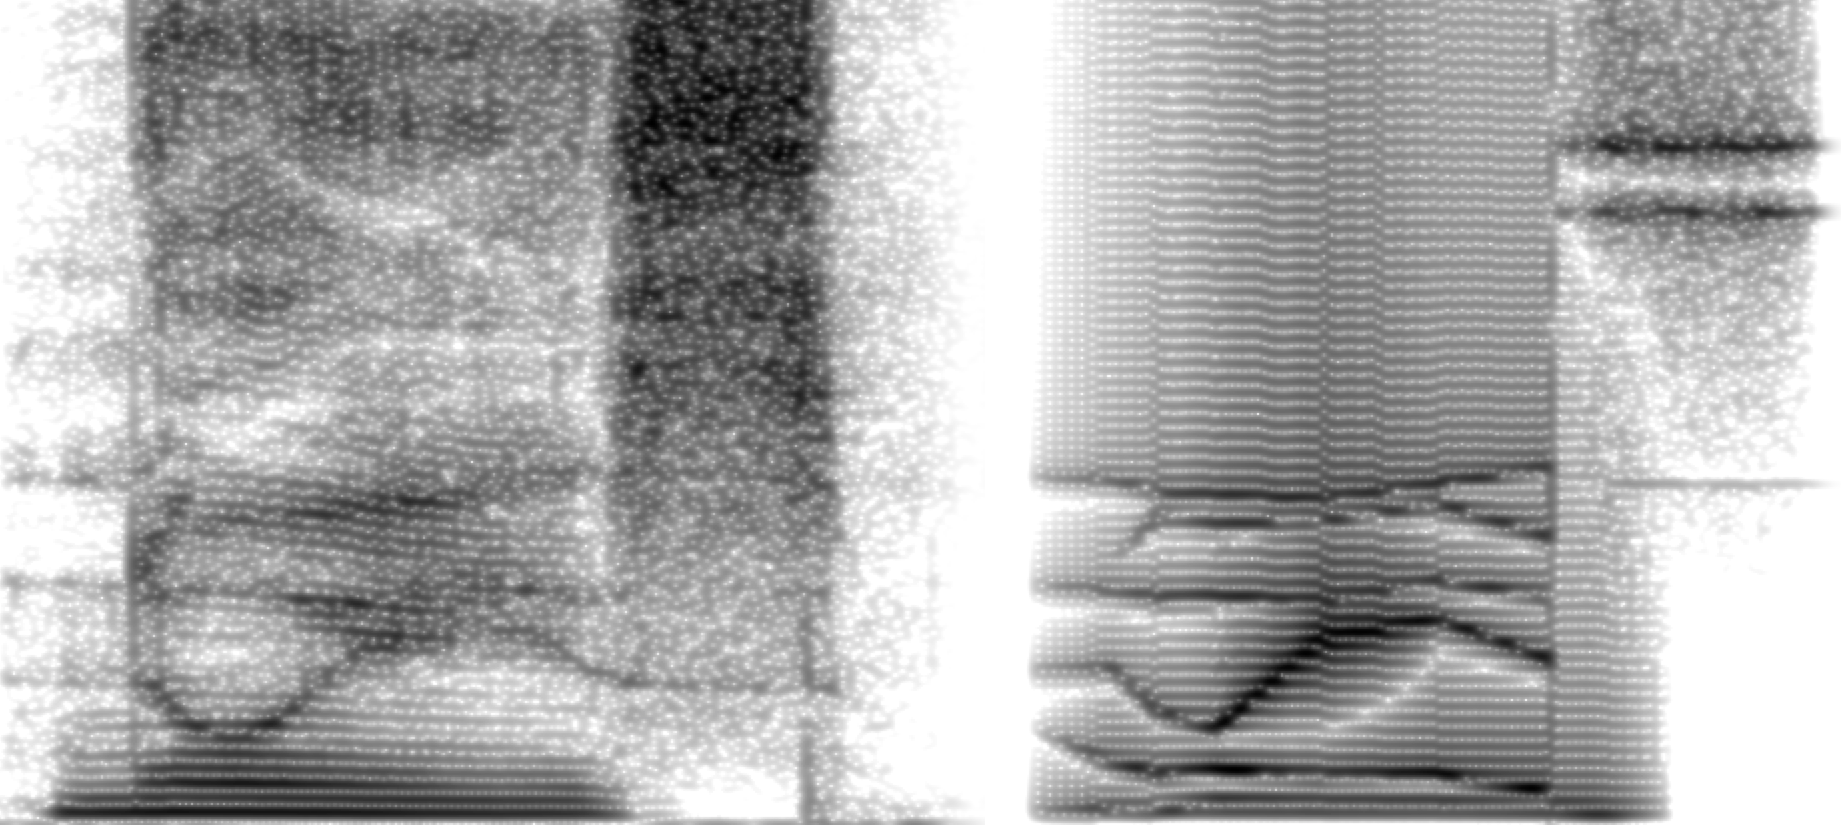
\includegraphics[width=0.5\textwidth]{noise_spectrograms.png}
	\caption{Comparison of spectrograms taken from Praat for \ipa{nɔɪz}. Reference (left) vs synthesised (right). 0-10kHz, 0.02 window size.}
	\label{fig:noise_spectrograms}
\end{figure}
%
Whilst writing this report I realised that I could have viewed the spectral slice in Praat which would have made direct analysis much easier, and fitting much more straightforward (see Figure \ref{fig:z_slice} below).
%
\begin{figure}[H] 
	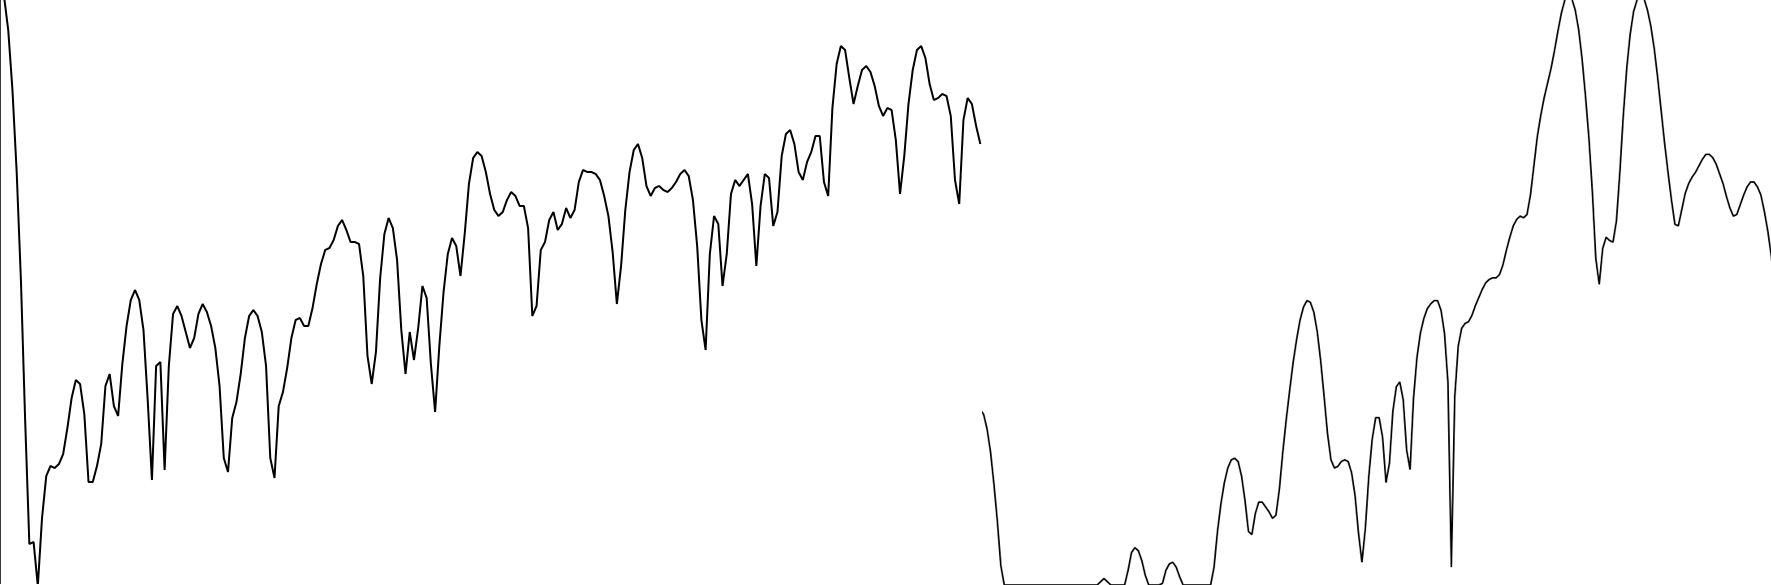
\includegraphics[width=0.5\textwidth]{z_slice.png}
	\caption{Comparison of of the spectral slice of \ipa{z} from 0-10kHz linear. There are more prominent peaks on the synthesised (right).}
	\label{fig:z_slice}
\end{figure}
%
Determining  LF-model parameters requires a lot of time. The additional parameters in the revised model \cite{Fant1995} provide further control over the spectrum: increasing $R_k$ raises relative level of voice fundamental. Increasing $R_g$ promotes the level of the second harmonic at the expense of the fundamental. This analysis starts to explore spectral qualities of specific voices, e.g. sonorous voices have relatively high $F_a$ of the order of \si{2000Hz} \cite{Fant1995}. Fant discusses a shape parameter, $R_d$, which predicts the other values, citing a 1994 publication that I was unable to locate a copy of \cite{Fant1994}. I tried to implement this as I felt it would make fitting parameters easier, however I had enormous problems matching up the ``statistical relations". The work in progress for this can be seen in the \obj{lfmodel\char`~} patch. I would like to complete this.

Using `typical' values for voice source parameters is difficult with my reference voice as I am a trans woman and my voice differs from typical male or female voices; for trans women there is a tendency for $F_3$ to be raised compared to male voices, with slower speech at reduced loudness and a higher $F_0$ \cite{Gunzburger1995}. This raises into question the `typical' LF parameters suggested for males or females in the literature.

The transitions between formant centre frequencies in my system are linear. This isn't true to formants in human speech, which have more gradual ramps between positions. See Figure \ref{fig:bout_non_linear_tx} below for an example. For my final word I compensated for this by having more interpolation points during the word and ramping between them. 
%
\begin{figure}[H] 
	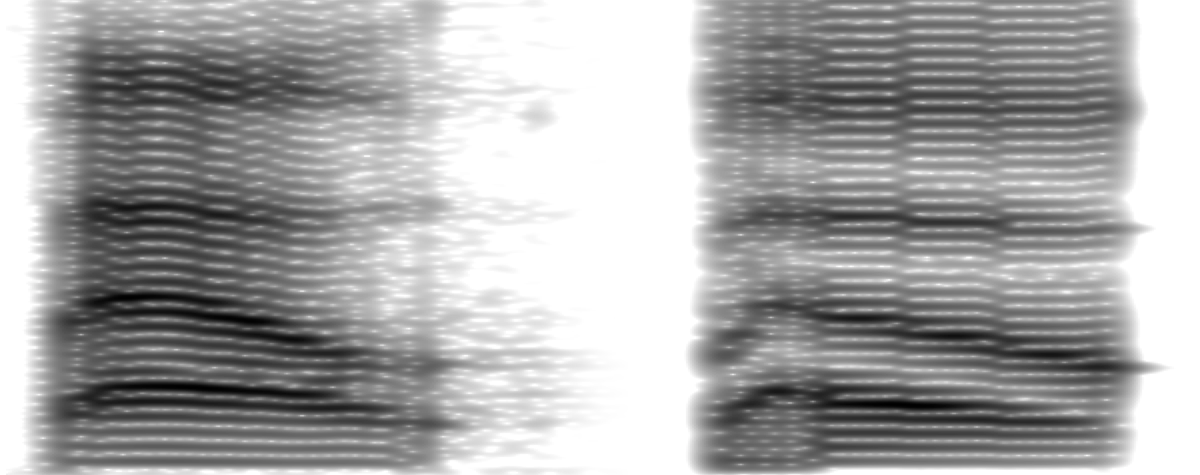
\includegraphics[width=0.5\textwidth]{bout_non_linear_tx.png}
	\caption{Non-linearity of $F_n$ transitions in Praat for \ipa{baʊt} reference (left) vs synthesised (right).}
	\label{fig:bout_non_linear_tx}
\end{figure}
%
In the real vocal tract the jet stream of frication noise is interrupted when the glottis is closed. To implement this I would need to integrate the glottal derivative and amplitude modulate the frication noise with this signal (the glottal flow). It may have been better if the frication noise bypassed the VTTF for vowels altogether, or used a different VTTF. This is because the `sound source' for fricatives is not the glottis but rather the area where the jet stream hits a wall, e.g. the teeth. Filtering this signal through the vocal tract is removes a lot of the signal too early.

My LF-model has four parameters changing every 1ms. A DSP cycle is 23µs at 44100kHz; on my machine this calculation takes 1310µs, which is a loss of resolution and exceeds the 1ms time grain. A computationally efficient alternative has been proposed and demonstrated to be perceptually equivalent in a listening tests \cite{Veldhuis1998}. This could be used.

As a final note, I had extensive problems implementing a flexible system in PD which has very limited metaprogramming abilities. Additionally, PD-extended had its last update four years ago and can be somewhat buggy on OS X. Rarely, the \obj{biquad\~} filters will become locked in an unstable state and the patch will need to be restarted (please do this if you hear an aggressive siren or chopping sound). I would love to implement in another system such as SuperCollider or a higher level programming language to really explore the possibilities.
